\subsubsection{„PolyBot“ sistema}

V. Shkapenyuk ir T. Suel aprašytas tinkle skirtinguose mazguose išskirstytas saityno peržiūros robotas, parašytas C++ ir Python programavimo kalbomis \cite{PolyBotArchitecture}.

Aprašyta architektūra (\ref{fig:polybot} schema) pasižymi peržiūros valdiklio komponentu, kuris gauna URL adresų užklausas ir paskirsto jas parsiuntimo komponentams \cite{PolyBotArchitecture}. Kiekvienas valdiklis gali komunikuoti daugiausiai su 8 parsiuntimo moduliais \cite{PolyBotArchitecture}. Peržiūros valdikliai tokioje architektūroje sukelia „butelio kaklelio“ efektą. Kitas apribojantis šios architektūros komponentas -- peržiūros programa (angl. -- \textit{Crawling Application}), kuri atsakinga už HTML dokumentų apdorojimą, peržiūros prioritizavimą ir žvalgytinų puslapių perdavimą valdikliui \cite{PolyBotArchitecture}. Kaip teigiama \cite{PolyBotArchitecture} šaltinyje, šis komponentas gali daugiausiai apdoroti 400 puslapių per sekundę.

\begin{figure}[htp!]
\hspace{-1cm}
\centering
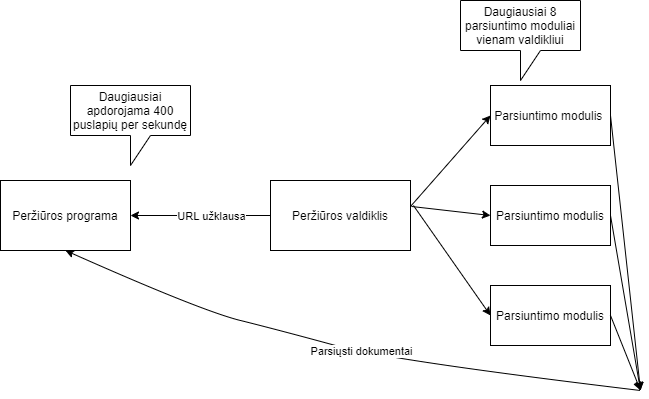
\includegraphics[scale=0.6]{img/plybot.png}
\caption{„Polybot“ peržiūros roboto architektūra}
\label{fig:polybot}
\end{figure}
